\begin{figure}[tbp]
\begin{center}
\includegraphics[width=0.48\textwidth]{compare_powv2d_z1z2.eps}
\end{center}
\vspace{-0.7cm}
\caption{(Top) The cross correlation r between $P_{v_z}$ and 
    $P_{\hat v_z^{fs}}$ calculated from foreground substracted field $\delta_{fs}$; 
    (Bottom) The cross correlation between $P_{v_z}$ and $P_{\hat v_z^{tide}}$ calculated from $\hat \kappa_c$. 
The contour line indicates $k^3 P(k)$.
}
\label{fig:v}
\end{figure}
We use six $N$-body simulations from the
$\mr{CUBEP}^3\mr{M}$ code \cite{2013:code}, each evolving $1024^3$ particles in a $(1.2\mr{Gpc}/h)^3$ box. 
We assume Hubble parameter $h=0.678$, baryon
density $\Omega_{b}=0.049$, dark matter density $\Omega_{c}=0.259$,
amplitude of primordial curvature power spectrum $A_s=2.139\times10^{-9}$ at 
$k_0=0.05\;\mr{Mpc}^{-1}$ and scalar spectral index $n_s=0.968$.
We analyse the outputs at redshift 1 and 2.

To ressemble realistic observations:

1. We import a cut off scale $k_c$, assume that modes with $k>k_c$ are not resolved.
This is reasonable for a filled aperture experiment, which
has good brightness sensitivity and an exponetially growing noise at small 
scales.
We choose $k_c=0.5\ h/\mr{Mpc}$ and $0.32 h/\mr{Mpc}$ respectively for $z=1$ and $z=2$ , which corresponds
to $\ell\sim1150$. 
This is generally realistic, judging from ongoing 21cm experiments like
CHIME \cite{2014SPIE.9145E..22B}\cite{2014SPIE.9145E..4VN}
and Tianlai \cite{2012IJMPS..12..256C}\cite{2015ApJ...798...40X}.

2. We use a high pass filter $W_{fs}(k_\parallel)=1-e^{-k_\parallel^2R_\parallel^2/2}$ to imitate the foreground substraction. 
We choose 
$R_\parallel=15\ \mr{Mpc}/h$ for $z=1$ and $R_\parallel=8\ \mr{Mpc}/h$ for $z=2$, which gives
$W_{fs}=0.5$ at
$k_\parallel=0.08\ \mr{Mpc}/h$ and $0.15\ \mr{Mpc}/h$ respectively. 
%This is realistic according to the condition of current 21cm observations 
%\cite{2013ApJ...763L..20M}\cite{Switzer13}.

The observed 21cm field after foreground subtraction is then given by 
\begin{eqnarray}
\label{eq:fs}
\delta_{fs}(\bm{k})=\delta(\bm{k})W_{fs}(k_\parallel)J(k_c-k),
\end{eqnarray}
where $\delta(\bm{k})$ is the original density field, 
%$W_{fs}$ accounts for 
%the effect of foreground subtraction and 
$J(x)$ equals 0 for $x<0$ and equals 1 elsewhere.

After that, we reconstruct the large scale fields $\hat \kappa_c$ from $\delta_{fs}$ via
cosmic tidal reconstruction. 
We use $\hat \kappa_c$ to obtain an estimate radial velocity field $\hat v_z^{tide}$ follow Eq.(\ref{eq:v}).
We reconstruct the kSZ signal $\hat \Theta^{tide}$ following Eq.(\ref{eq:ksz}) and compare it with kSZ signal.

To show the effects of tidal reconstruction, we go through the same procedure for $\delta_fs$ and get $\hat \Theta{fs}$. 
